% Final report (Phase 2, issue #63). Each section lives in sections/<name>.tex and is
% written by its owner (see README.md and the section issues); this file only sets up
% the template and the order, which follows the Phase 2 brief.
% Build from this folder: `tectonic main.tex`, or pdflatex + bibtex (e.g. Overleaf).

\documentclass[conference]{IEEEtran}

\usepackage{iftex}
\ifXeTeX
  % Tectonic and xelatex: Times-like text to match pdflatex's IEEEtran output.
  \usepackage{fontspec}
  \defaultfontfeatures{Extension=.otf, UprightFont=*-regular, BoldFont=*-bold,
    ItalicFont=*-italic, BoldItalicFont=*-bolditalic}
  \setmainfont{texgyretermes}
  \setsansfont{texgyreheros}
  \setmonofont{texgyrecursor}
\fi
\usepackage{cite}
\usepackage{amsmath,amssymb}
\usepackage{graphicx}
\usepackage{url}
\usepackage{booktabs}
\usepackage{array}
\usepackage{tikz}
\usetikzlibrary{arrows.meta,positioning}
% Load last: makes the repository and video URLs and the cross-references
% clickable, and fills in the PDF's title and author fields.
\usepackage[hidelinks]{hyperref}
\hypersetup{
  pdftitle={A Parameterized Output-Stationary Systolic Array for Fixed-Point Matrix Multiplication: Final Design and Evaluation},
  pdfauthor={Gokul VKS, Milind Bansal, Isha Tomar, Yashi Agrawal, Mohammad Affan Anas},
  pdfkeywords={systolic array, matrix multiplication, tiling, hardware accelerator, FPGA synthesis, Verilog}}

% Figures come from this folder, from the committed results and from the
% architecture diagrams.
\graphicspath{{figures/}{../../results/phase2/figures/}{../../results/phase2/waveforms/}{../../results/phase1/waveforms/}{../../docs/architecture/png/}}

% Sections that other pull requests add are input only once they exist, so the
% report builds at every step. Assembly (#63) replaces these with plain \input.
\newcommand{\inputifexists}[1]{\IfFileExists{#1.tex}{\input{#1}}{}}

\begin{document}

\title{A Parameterized Output-Stationary Systolic Array\\
for Fixed-Point Matrix Multiplication:\\
Final Design and Evaluation}

\author{\IEEEauthorblockN{Gokul VKS, Milind Bansal, Isha Tomar, Yashi Agrawal and Mohammad Affan Anas}
\IEEEauthorblockA{Newton School of Technology, Rishihood University\\
Code and results: \url{https://github.com/vks-g/systolic-matmul-accelerator}\\
Phase~1 prototype video: \url{https://drive.google.com/drive/folders/1d-p1YpFjd7gjbm1XGEC8u5PCso8LQxUw}}}

\maketitle

% Abstract and index terms (final report #63).
% Draft: the speed-ups are the cycle model's (docs/spec.md section 11). At assembly,
% replace them with the measured values (#69, #64) and add the synthesis results (#75).

\begin{abstract}
Matrix multiplication dominates the run time of neural-network inference and many signal-processing workloads, and on general-purpose processors its cost is set by data movement rather than arithmetic. This paper presents the final design and evaluation of a matrix-multiplication accelerator built on an output-stationary systolic array. An $N \times N$ grid of processing elements, $4 \times 4$ by default, multiplies signed 8-bit fixed-point operands and accumulates each element of the result in place in a 32-bit register. The host sets the inner length of each run, from 1 to 16, and can start a run that adds onto the previous result instead of clearing it. These two additions leave the array itself unchanged, yet they let a host multiply matrices of any size, one $N \times N$ tile of the result and one chunk of the inner dimension at a time. The design is synthesizable, parameterized Verilog-2005 with a written timing contract: a run with inner length $k$ is busy for $k + 2N$ cycles. To measure the benefit of the array rather than derive it, we built a sequential baseline with one multiply-accumulate unit and the same host interface, which is busy for $N^2 k$ cycles. The array needs 5.3 times fewer busy cycles than the baseline for $k = 4$ and 10.7 times fewer for $k = 16$, but loading the operands through one-element ports limits the end-to-end speed-up of an $8 \times 8 \times 8$ product to 2.7. Both designs are synthesized for a Lattice ECP5 FPGA with the open-source Yosys and nextpnr tools, and we report their resources and maximum clock frequency. Self-checking testbenches for every module, a Python golden model and continuous integration verify the design, including inner lengths other than $N$ and tiled products larger than the array.
\end{abstract}

\begin{IEEEkeywords}
systolic array, matrix multiplication, hardware accelerator, output-stationary dataflow, tiling, fixed-point arithmetic, FPGA synthesis, Verilog
\end{IEEEkeywords}


% Introduction (issue #5; final report #63).
% Still the Phase 1 text: rewritten in #63 once the Phase 2 results are in.

\section{Introduction}
Matrix multiplication is the core operation of fully connected and convolutional neural-network layers, of transformers, and of many filters and transforms in signal processing. Multiplying two $N \times N$ matrices takes $N^3$ multiply-accumulate (MAC) operations, and each operand is used $N$ times. A general-purpose processor fetches those operands again and again through its memory hierarchy, and the energy of that data movement exceeds the energy of the arithmetic by orders of magnitude~\cite{horowitz2014energy, sze2017efficient}. Dedicated hardware that keeps operands close to many parallel MAC units is therefore the standard way to accelerate this workload.

A systolic array is a regular grid of identical processing elements (PEs), each connected only to its neighbours, through which data moves in step with a single clock~\cite{kung1979systolic, kung1982systolic}. Each operand is read from memory once and then reused as it passes from PE to PE, so the array performs many operations per memory access. Its short, local wires make it straightforward to scale and to lay out. The same structure is at the heart of production accelerators such as Google's Tensor Processing Unit~\cite{jouppi2017tpu} and of open-source generators such as Gemmini~\cite{genc2021gemmini}.

This project designs, verifies and evaluates a systolic-array matrix-multiplication accelerator in two phases. Phase~1, reported here, delivers a working register-transfer-level (RTL) prototype:
\begin{itemize}
\item a parameterized $N \times N$ output-stationary systolic array, $4 \times 4$ by default, for signed 8-bit fixed-point operands with 32-bit accumulators;
\item input skew buffers, an output buffer and a controller, which together give the array a simple host interface: write $A$ and $B$, pulse \texttt{start}, read $C$;
\item a written specification that fixes every port, the input skew, and a compute latency of $K + 2N - 2$ cycles before any RTL was written, so the five team members could build and test their modules in parallel;
\item a verification flow in which every module has a self-checking testbench, a Python golden model provides the expected results, and continuous integration lints and simulates every pull request.
\end{itemize}
Phase~2 will synthesize the design, measure its speed-up against a sequential baseline in RTL, and extend it to matrices larger than the array.

Section~II reviews systolic arrays, their dataflows and published accelerators. Section~III describes the architecture, the PE and multiply-accumulate unit, the dataflow and the controller. Section~IV presents the verification methodology and Section~V the status of the prototype. Section~VI concludes with the plan for Phase~2, and Section~VII lists the contributions of each team member.

\inputifexists{sections/literature_review}  % #74

% Proposed Solution
% Proposed solution: system architecture overview (issue #5; final report #63).
% Fig. system.png comes from docs/architecture/ (#18, updated in #76); re-exporting
% it there updates the report.

\section{Proposed Solution}
\subsection{Architecture Overview}
The accelerator computes products of signed $\mathrm{DATA\_W}$-bit fixed-point matrices. One run multiplies an $N \times k_{\mathrm{len}}$ block of $A$ by a $k_{\mathrm{len}} \times N$ block of $B$:
\begin{equation}
C[i][j] = \sum_{k=0}^{k_{\mathrm{len}}-1} A[i][k]\,B[k][j],
\label{eq:matmul}
\end{equation}
where the host chooses the inner length $k_{\mathrm{len}}$ for each run, from 1 to $K_{\max}$. A run can also \emph{accumulate}, adding its products onto the result of the previous run instead of starting from zero. With these two features the host can multiply matrices of any size, one $N \times N$ tile of $C$ and one chunk of the inner dimension at a time (Section~III-E). Table~\ref{tab:params} lists the parameters. Every module takes them as Verilog parameters, so the array size, the operand storage and the data widths change in one place.

\begin{table}[t]
\centering
\caption{Design parameters}
\label{tab:params}
\footnotesize
\begin{tabular}{@{}llc@{}}
\toprule
Parameter & Meaning & Default \\
\midrule
$N$ & array size; $C$ is computed in $N \times N$ tiles & 4 \\
$K_{\max}$ & largest inner length of one run & 16 \\
$\mathrm{DATA\_W}$ & operand width, signed & 8 \\
$\mathrm{ACC\_W}$ & accumulator and result width, signed & 32 \\
$\mathrm{FRAC\_W}$ & fractional bits of the Q-format reading & 0 \\
\midrule
$k_{\mathrm{len}}$ & inner length of a run, set by the host & 1 to 16 \\
$T$ & compute cycles of a run, $k_{\mathrm{len}} + 2N - 2$ & 7 to 22 \\
\bottomrule
\end{tabular}
\end{table}

\begin{figure*}[t]
\centering
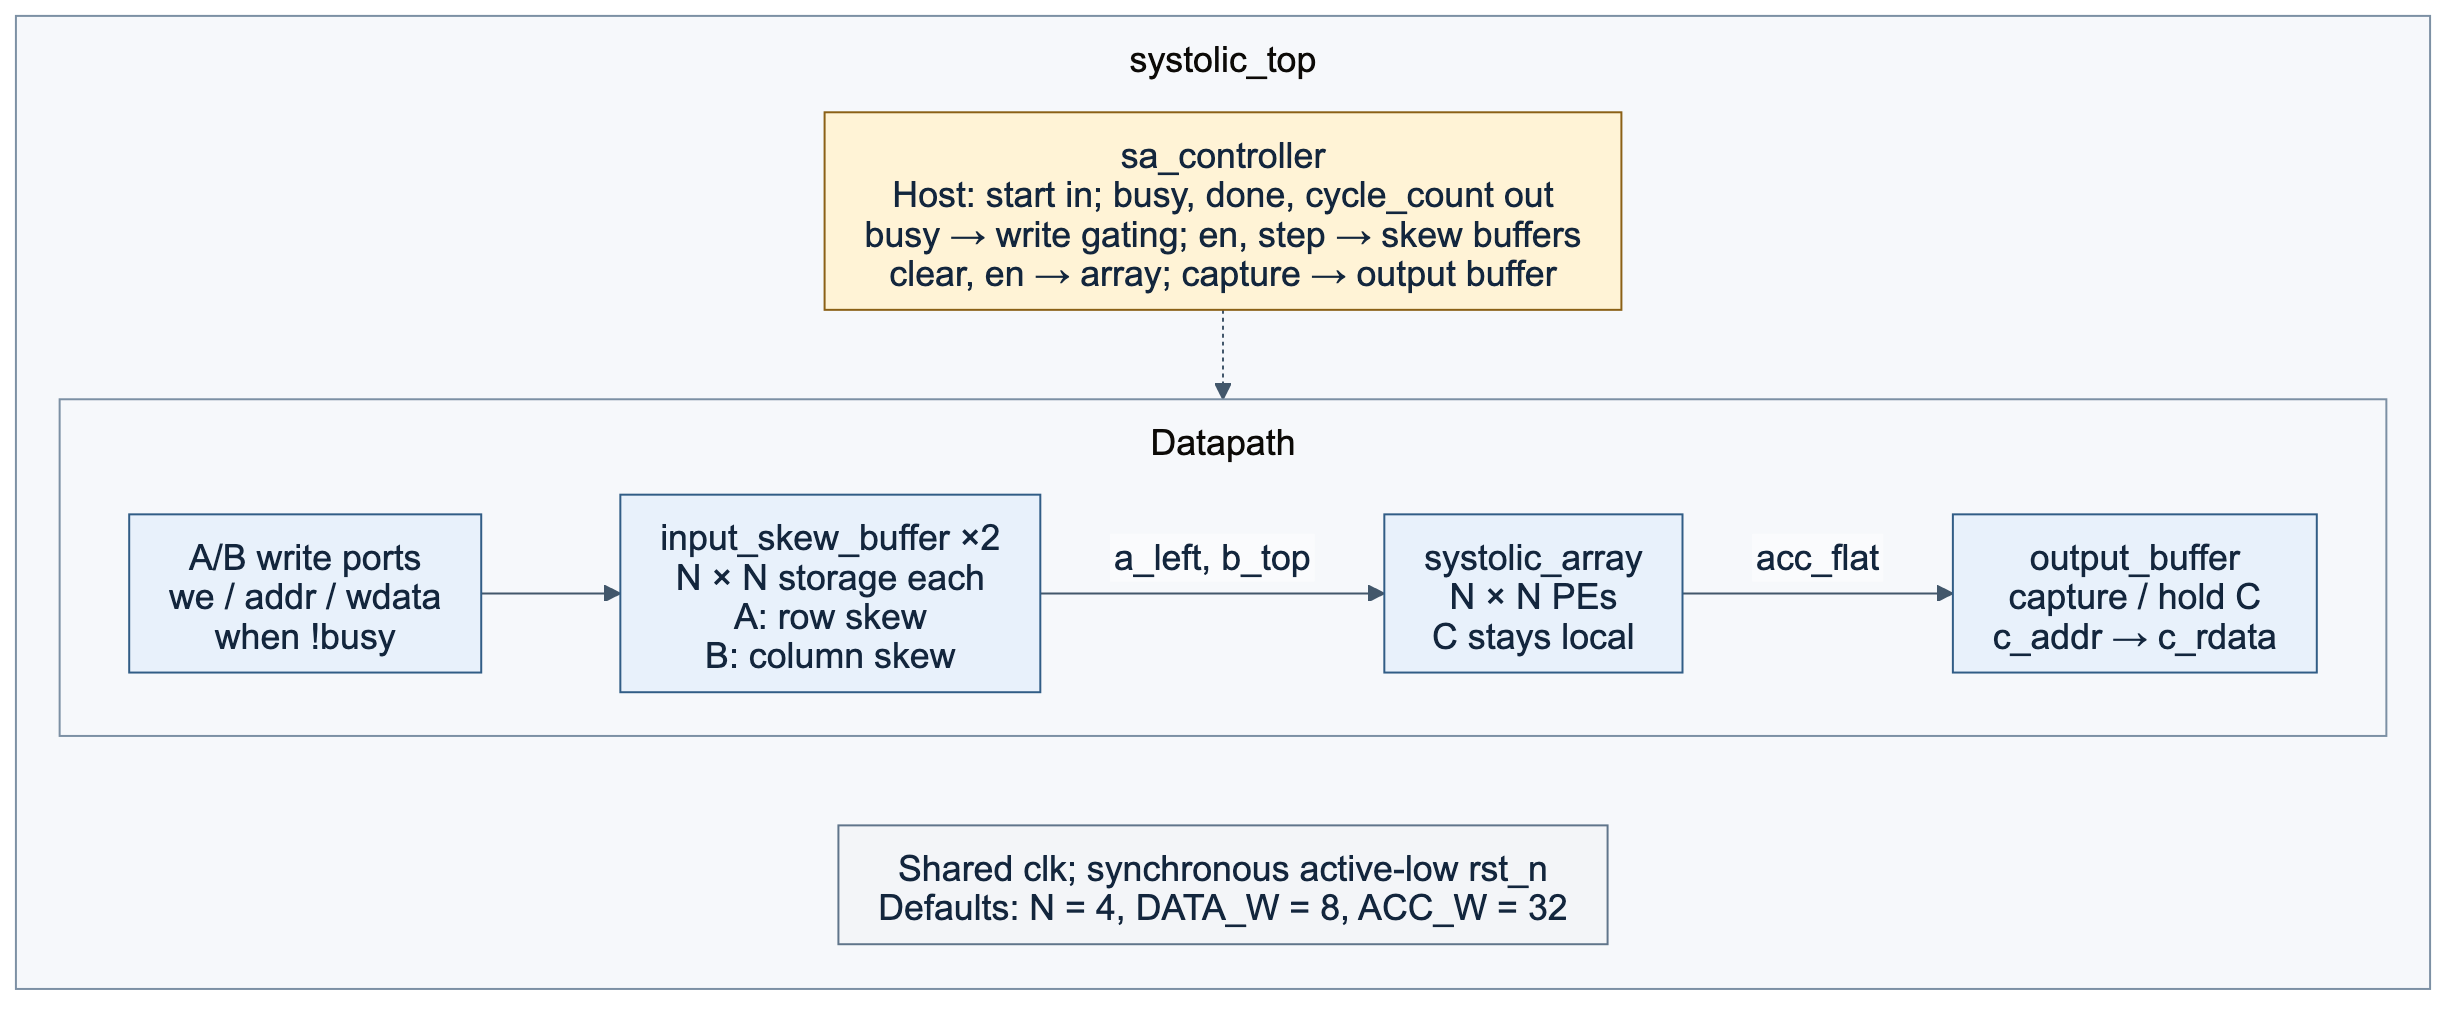
\includegraphics[width=\textwidth]{system.png}
\caption{System architecture. Solid arrows carry data and dashed arrows carry controller signals. Host writes reach the input skew buffers only while \texttt{busy} is low. Each buffer stores one operand block and selects its skewed lanes from the compute step and the run's inner length. The controller samples $k_{\mathrm{len}}$ and \texttt{accumulate} with \texttt{start}, clears the array unless the run accumulates, enables it for $T$ steps and then captures the accumulators into the output buffer, which serves the read port.}
\label{fig:system}
\end{figure*}

The design has five blocks behind one host interface, shown in Fig.~\ref{fig:system}:
\begin{itemize}
\item \textbf{Two input skew buffers.} The A buffer stores $N$ rows of $K_{\max}$ elements and the B buffer $K_{\max}$ rows of $N$ elements. During a run, the A buffer drives element $k$ of row $i$ into the left edge in step $i + k$, and the B buffer drives element $k$ of column $j$ into the top edge in step $j + k$, for every $k < k_{\mathrm{len}}$. Elements beyond $k_{\mathrm{len}}$ are never sent, so old data in the buffers needs no clearing.
\item \textbf{The systolic array.} An $N \times N$ grid of PEs. PE $(i,j)$ multiplies the operands that reach it, adds the product to its accumulator, which holds $C[i][j]$, and passes $A$ to the right and $B$ down one cycle later. The array is the same as in Phase~1: the inner length only changes how long operands keep arriving. The PE is described in Section~III-B and the skew in Section~III-C.
\item \textbf{The output buffer.} Copies all $N^2$ accumulators in one cycle when a run ends, and serves them to the host through a read port. The previous result therefore stays readable while the next run computes.
\item \textbf{The controller.} A five-state machine that samples $k_{\mathrm{len}}$ and \texttt{accumulate}, clears the array unless the run accumulates, runs the $T$ compute steps, and signals the capture and the end of the run (Section~III-D).
\end{itemize}

The host sees a small matrix data interface. It writes $A$ and $B$ one element at a time through two write ports, $A[r][k]$ at address $rK_{\max} + k$ and $B[k][c]$ at address $kN + c$, sets $k_{\mathrm{len}}$ and \texttt{accumulate}, pulses \texttt{start}, waits for \texttt{done}, and reads $C$ one element at a time through the read port. A \texttt{start} whose $k_{\mathrm{len}}$ is 0 or above $K_{\max}$ is ignored, and \texttt{busy} stays low, so the host can see that it was rejected. While \texttt{busy} is high, writes are ignored, so the operands of a running product cannot change. Between runs $A$ and $B$ keep their contents, so a host can replace one operand and start again. A \texttt{cycle\_count} output reports how many cycles the last run took, which the testbenches use to check the latency.

A normal run spends one cycle clearing every accumulator and forwarding register, then $T = k_{\mathrm{len}} + 2N - 2$ compute steps in which the skewed operands cross the array and every PE adds its $k_{\mathrm{len}}$ products, and one more cycle copying the accumulators into the output buffer before \texttt{done} rises. \texttt{busy} is therefore high for $k_{\mathrm{len}} + 2N$ cycles: 12 for $k_{\mathrm{len}} = 4$ and 24 for $k_{\mathrm{len}} = K_{\max} = 16$. An accumulate run skips the clear and takes one cycle fewer.

The sequential baseline that the results compare against, \texttt{seq\_matmul}, has exactly the same ports and address map, so the same testbenches and the live demonstration drive both designs. It contains one multiplier and one adder with the same arithmetic as the PE, computes $C$ one element at a time, and is busy for $N^2 k_{\mathrm{len}}$ cycles per run.

The array performs $N^2 = 16$ MACs per cycle at its peak. A run performs $N^2 k_{\mathrm{len}}$ MACs in $T$ compute cycles, against $N^2 k_{\mathrm{len}}$ cycles for the baseline, a compute speed-up of $N^2 k_{\mathrm{len}}/T$: 6.4 for $k_{\mathrm{len}} = 4$ and 11.6 for $k_{\mathrm{len}} = 16$. Each PE is busy for $k_{\mathrm{len}}$ of the $T$ cycles, so utilization rises from 40\,\% at $k_{\mathrm{len}} = 4$ to 72.7\,\% at $k_{\mathrm{len}} = 16$, because the wavefront's $2N - 2$ cycles of fill and drain are paid once per run. Loading a run's operands through the one-element ports takes $N k_{\mathrm{len}}$ cycles, more than the run itself, so end to end the ports, not the array, limit throughput (Section~V).

The arithmetic is exact integer arithmetic. The 32-bit accumulators cannot overflow for any inner dimension below 131{,}072, counted across all the chunks of a tiled product (Section~III-B), so the datapath needs no rounding or saturation. Operands can also be read as Q-format fixed-point numbers with $\mathrm{FRAC\_W}$ fractional bits, and each element of $C$ then has $2\,\mathrm{FRAC\_W}$ fractional bits. This changes only how the numbers are read, not the hardware.

% Proposed solution: processing element and MAC microarchitecture (issue #9; final-report update in #67).

\subsection{Processing Element and MAC Unit}
Each processing element (PE) owns one output element $C[i][j]$. It holds a multiply-accumulate unit (MAC) and two forwarding registers. The MAC multiplies two signed 8-bit operands into a 16-bit product, sign-extends that product to a 32-bit accumulator, and adds it to the running sum in every enabled cycle. The product is formed at its natural width before the sign extension, so the sign bit is never read as zero. Clear has priority over enable, and reset behaves like clear.

The PE also registers its operands. The left operand $a$ is copied to the right neighbour and the top operand $b$ to the neighbour below, one enabled cycle later. Each operand therefore moves one PE per cycle, which is what lets the skewed inputs meet at PE $(i,j)$ in the cycle that the term $A[i][k]B[k][j]$ needs. Fig.~\ref{fig:pe-wave} shows both behaviours in the PE testbench: the forwarded operands trail the inputs by one cycle, and four products accumulate to the expected dot product of 70.

\begin{figure*}[t]
\centering
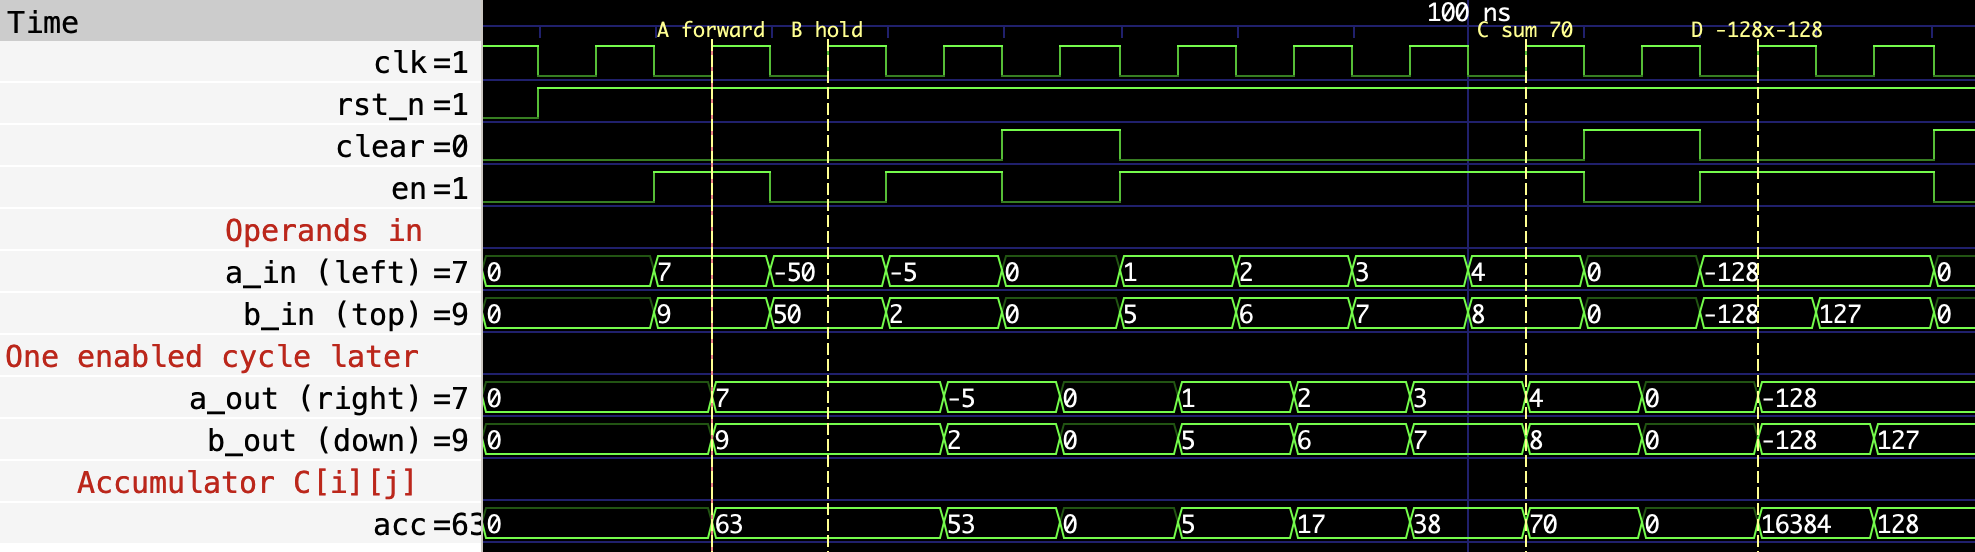
\includegraphics[width=\textwidth]{pe.png}
\caption{One PE in simulation (\texttt{tb\_pe}, GTKWave). Each operand leaves on \texttt{a\_out} and \texttt{b\_out} one enabled cycle after it arrives (A) and holds while \texttt{en} is low (B). The accumulator sums $1\cdot5 + 2\cdot6 + 3\cdot7 + 4\cdot8 = 70$ over $K = 4$ steps (C), and $-128 \times -128$ gives 16{,}384 (D).}
\label{fig:pe-wave}
\end{figure*}

The accumulator width follows from the largest possible sum. For $K = N = 4$ the largest magnitude is $K \cdot 2^{2\cdot\mathrm{DATA\_W}-2} = 4 \cdot 2^{14} = 65{,}536$, reached when every operand is $-128$. That needs 18 bits, so a 32-bit accumulator cannot overflow for any $K$ below 131{,}072. The datapath therefore does not saturate. Rounding and saturating back to 8 bits are left for Phase 2.
                     % #67
% Proposed solution: output-stationary dataflow and input skewing (issue #13; final-report update in #71).

\subsection{Dataflow and Input Skewing}
The array is output-stationary: PE $(i,j)$ keeps $C[i][j]$ in its accumulator for the whole run, and only the operands move. Row $i$ of $A$ enters the left edge at PE $(i,0)$ and moves one PE to the right per cycle. Column $j$ of $B$ enters the top edge at PE $(0,j)$ and moves one PE down per cycle. Results never move during the computation, so the output buffer can copy all $N^2$ of them in one cycle when it ends.

The two operands of a product must reach a PE in the same cycle. Number the compute cycles $t = 0, 1, \ldots, T-1$. In step $t$ the skew buffers put $A[i][t-i]$ on lane $i$ of the left edge and $B[t-j][j]$ on lane $j$ of the top edge, and zero when the index falls outside $0 \le k < K$; Table~\ref{tab:skew} lists them for $N = 4$. Each PE adds one cycle of delay in each direction, so in step $t$ PE $(i,j)$ receives
\begin{equation}
a = A[i][t-i-j], \qquad b = B[t-i-j][j].
\end{equation}
Both carry the same index $k = t - i - j$. PE $(i,j)$ therefore adds the term $A[i][k]\,B[k][j]$ of~\eqref{eq:matmul} in step $t = i + j + k$, and it receives zeros, which add nothing, in every other step.

The compute length follows from the last term. PE $(i,j)$ is busy from step $i+j$ to step $i+j+K-1$, so the last PE, $(N{-}1,N{-}1)$, adds its last term in step $K + 2N - 3$, and
\begin{equation}
T = K + 2N - 2,
\end{equation}
which is 10 for $N = K = 4$. The PEs that are busy in one step lie on anti-diagonals: in step 3, PE $(0,0)$ adds its term $k = 3$ while PE $(3,0)$ adds its term $k = 0$. The edges go quiet after step $K + N - 2 = 6$, but the last operands are still crossing the array until step 9.

\begin{table}[t]
\centering
\caption{Edge inputs in each compute step for $N = K = 4$ ($\cdot$ is zero)}
\label{tab:skew}
\scriptsize
\setlength{\tabcolsep}{3.2pt}
\begin{tabular}{@{}c|cccc|cccc@{}}
\toprule
 & \multicolumn{4}{c|}{left edge, lane $i$} & \multicolumn{4}{c}{top edge, lane $j$} \\
$t$ & 0 & 1 & 2 & 3 & 0 & 1 & 2 & 3 \\
\midrule
0 & $A_{00}$ & $\cdot$ & $\cdot$ & $\cdot$ & $B_{00}$ & $\cdot$ & $\cdot$ & $\cdot$ \\
1 & $A_{01}$ & $A_{10}$ & $\cdot$ & $\cdot$ & $B_{10}$ & $B_{01}$ & $\cdot$ & $\cdot$ \\
2 & $A_{02}$ & $A_{11}$ & $A_{20}$ & $\cdot$ & $B_{20}$ & $B_{11}$ & $B_{02}$ & $\cdot$ \\
3 & $A_{03}$ & $A_{12}$ & $A_{21}$ & $A_{30}$ & $B_{30}$ & $B_{21}$ & $B_{12}$ & $B_{03}$ \\
4 & $\cdot$ & $A_{13}$ & $A_{22}$ & $A_{31}$ & $\cdot$ & $B_{31}$ & $B_{22}$ & $B_{13}$ \\
5 & $\cdot$ & $\cdot$ & $A_{23}$ & $A_{32}$ & $\cdot$ & $\cdot$ & $B_{32}$ & $B_{23}$ \\
6 & $\cdot$ & $\cdot$ & $\cdot$ & $A_{33}$ & $\cdot$ & $\cdot$ & $\cdot$ & $B_{33}$ \\
7--9 & $\cdot$ & $\cdot$ & $\cdot$ & $\cdot$ & $\cdot$ & $\cdot$ & $\cdot$ & $\cdot$ \\
\bottomrule
\end{tabular}
\end{table}

Each input skew buffer stores one $N \times N$ matrix, written row-major by the host before \texttt{start}. During compute it selects its lanes combinationally from the controller's \texttt{step}: lane $l$ carries $M[l][t-l]$ for $A$, whose lanes are rows, and $M[t-l][l]$ for $B$, whose lanes are columns. One module serves both edges through a parameter. The buffer compares $t \ge l$ before it subtracts, so the index never wraps around. Selecting from stored operands rather than shifting them through delay registers means the host may write the matrices in any order, and both matrices stay in place for the next run.
                   % #71
% Proposed solution: controller FSM (issue #9; final-report update in #67).

\subsection{Controller}
The controller sequences one matrix multiplication through five states, shown in Fig.~\ref{fig:fsm}. Its outputs are decoded from the state register, so they change only on clock edges. In \texttt{CLEAR} the accumulators and forwarding registers are zeroed. \texttt{COMPUTE} then runs for $T = K + 2N - 2$ cycles, which is 10 for $N = 4$: the last PE, $(N{-}1, N{-}1)$, adds its last product in step $T-1$. \texttt{CAPTURE} copies every accumulator into the output buffer, and \texttt{DONE} holds the result while \texttt{done} is high. A \texttt{start} pulse is accepted only in \texttt{IDLE} and \texttt{DONE} and is ignored while the array is busy. A full run keeps the controller busy for $K + 2N = 12$ cycles, and \texttt{cycle\_count} reports that number when the run ends.

\begin{figure}[t]
\centering
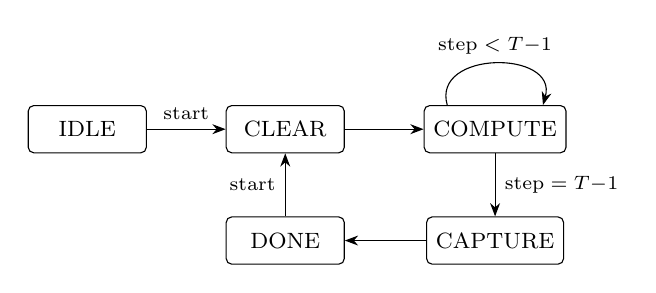
\begin{tikzpicture}[>=Stealth, font=\footnotesize,
  st/.style={draw, rounded corners=2pt, minimum width=15mm, minimum height=6mm, align=center},
  lab/.style={font=\scriptsize}]
  \node[st] (idle) {IDLE};
  \node[st, right=10mm of idle] (clear) {CLEAR};
  \node[st, right=10mm of clear] (comp) {COMPUTE};
  \node[st, below=8mm of comp] (cap) {CAPTURE};
  \node[st, below=8mm of clear] (done) {DONE};
  \draw[->] (idle) -- node[above, lab] {start} (clear);
  \draw[->] (clear) -- (comp);
  \draw[->] (comp) -- node[right, lab] {$\mathrm{step} = T{-}1$} (cap);
  \draw[->] (cap) -- (done);
  \draw[->] (done) -- node[left, lab] {start} (clear);
  \draw[->] (comp.north west) ++(3mm,0) .. controls +(-2mm,7mm) and +(2mm,7mm) .. node[above, lab] {$\mathrm{step} < T{-}1$} ([xshift=-3mm]comp.north east);
\end{tikzpicture}
\caption{Controller state-transition diagram. \texttt{busy} is high in \texttt{CLEAR}, \texttt{COMPUTE} and \texttt{CAPTURE}.}
\label{fig:fsm}
\end{figure}
                 % #67
% Proposed solution: run-time inner length, accumulate runs and tiling (issue #63).
% Follows docs/spec.md sections 7 and 12. The tiling figure from #76 goes here
% once it is exported to docs/architecture/png/.

\subsection{Tiling Products Larger than the Array}
The array holds one $N \times N$ tile of $C$, and the operand buffers hold at most $K_{\max}$ elements of the inner dimension. A host multiplies an $M \times K$ matrix $A$ by a $K \times P$ matrix $B$ of any size by splitting the product into runs that fit:
\begin{enumerate}
\item It splits $C$ into $\lceil M/N \rceil \cdot \lceil P/N \rceil$ output tiles of $N \times N$ elements.
\item It splits the inner dimension into $c = \lceil K/K_{\max} \rceil$ chunks. Every chunk has $K_{\max}$ elements except possibly the last.
\item For each tile, it runs the chunks in order. Before each run it writes the $N \times k_{\mathrm{len}}$ block of $A$ and the $k_{\mathrm{len}} \times N$ block of $B$ for that tile and chunk. Rows of $A$ beyond $M$ and columns of $B$ beyond $P$ are written as zeros, because the buffers keep their old contents. The first chunk starts normally, and every later chunk starts with \texttt{accumulate} high.
\item After the last chunk it reads the tile and keeps the rows below $M$ and the columns below $P$.
\end{enumerate}

The accumulate start is what makes this cheap. The dataflow is output-stationary, so the partial sums of a tile stay in their PEs between chunks: no partial sum leaves the array, and only the finished tile is read. Skipping the clear step is safe. In the last step of any run, every PE that feeds a neighbour holds operands with $k \geq k_{\mathrm{len}}$, which entered the array as zeros, so the forwarding registers are already empty when the next run starts. Only the accumulators carry over. The zero padding at the edges costs the same time as useful work, as it does on the TPU~\cite{jouppi2017tpu}.

A tile of a product with $c$ chunks takes one normal run and $c - 1$ accumulate runs, so the array is busy for
\begin{equation}
\sum_{\text{chunks}} \left(k_{\mathrm{len}} + 2N\right) - (c - 1) = K + c\,(2N - 1) + 1
\label{eq:tilebusy}
\end{equation}
cycles per tile. The sequential baseline, driven through the same ports and the same procedure, is busy for $N^2 K$ cycles per tile. In both designs, loading the operands takes $NK$ cycles per tile and reading the finished tile another $N^2$. For an $8 \times 8$ by $8 \times 8$ product on the default $4 \times 4$ array, the four tiles keep the array busy for 64 cycles against 512 for the baseline, a predicted speed-up of 8.0. Counting the loading, the start pulses and the readout, the totals are 260 and 708 cycles, a speed-up of only 2.7. Section~V compares these predictions with the measured cycle counts.


% Verification methodology and toolchain (issue #20; final-report update in #78).

\section{Verification Methodology}
Verification checks both the values of $C=AB$ and the timing and handshake
contract in \path{docs/spec.md}. Tests progress from individual modules to
the array and the complete accelerator, so a failure can be traced to an
arithmetic, forwarding, skew or control boundary.

\subsection{Tool Flow}
The synthesizable Verilog-2005 RTL first passes static checks with
Verilator~\cite{verilator2026guide}. The \texttt{make lint} target discovers all
RTL files and runs \texttt{--lint-only -Wall}, selecting each module as a
top and using the Verilog-2005 language setting. Warnings fail the target;
intentional unused signals have local waivers with explanations.

The \texttt{make test} target generates golden vectors, compiles each
\path{tb/tb_*.v} with Icarus Verilog using \texttt{-g2005 -Wall}, and runs
the resulting executable with \texttt{vvp}~\cite{icarus2026simulation}.
Testbenches dump VCD waveforms into \path{build/}. GTKWave provides manual
inspection of the operand wavefront, accumulator updates and controller
transitions~\cite{gtkwave2026docs}; saved layouts are in \path{sim/waves/}.
The \texttt{make waves} target reruns the top-level test and opens its VCD
in the selected viewer. Waveform inspection supplements the automated
comparisons. Synthesis, resource counts and maximum-frequency measurement
are Phase~2 work and are not part of this simulation flow.

\subsection{Hierarchical Testbenches}
The MAC test checks signed products, including $-128\times-128$ and
$-128\times127$, an accumulation chain, reset, clear priority and holding
with enable low. The PE test adds the one-enabled-cycle forwarding delay
and checks that both forwarding registers hold and clear with the
accumulator. Input-buffer tests compare every A and B lane at each step
with the spec's skew table; output-buffer tests check parallel capture,
holding the previous result and readout at every address.

Controller tests check the state sequence, busy-state rejection of
\texttt{start}, restart from \texttt{DONE}, mid-run reset and the exact
compute and busy lengths for $N=3$ and $N=4$. Array tests drive skewed
operands at the edges and check every PE's partial sum after each compute
edge, as well as final results, stalls and restart. They exercise both
array sizes, catching row/column indexing and fill/drain errors that a
single final-result comparison could miss.

The end-to-end test loads operands through the host ports and compares
every output element with golden vectors. It also checks ignored writes
while busy, back-to-back runs, replacing only one operand matrix,
preservation of the previous $C$ until capture, and reset during a run.
For each golden case it counts busy cycles and checks
\texttt{cycle\_count}: both must equal $K+2N$, or 12 for $N=K=4$.
The CSV in \path{results/phase1/cycle_counts.csv} records these measurements;
its compute-cycle field is derived by subtracting the one CLEAR and one
CAPTURE cycle. The controller tests check the compute interval directly
against $T=K+2N-2$, which is 10 cycles at the default size.

\subsection{Golden Results and Directed Cases}
The Python reference in \path{model/golden_model.py} computes signed
matrix products with NumPy integer arithmetic and checks operand and
result ranges. A separate cycle-level model starts with zero forwarding
registers and accumulators, applies the specified input skew, and advances
operands one PE per cycle. The vector generator refuses to write its
files unless this model agrees with the mathematical product after
exactly $T$ steps. Expected results therefore come from the reference or
hand-worked values, rather than recorded RTL output.

The default vector set contains six directed cases---identity, zero,
all ones, maximum negative operands, mixed signed extremes and a known
product with $A=1,\ldots,16$ in row-major order and $B=A^{\mathsf T}$---plus
100 random cases spanning the signed 8-bit range. The golden-vector seed
is 1; array tests use seeds 1 and 2 for $N=4$ and $N=3$. Seeds are printed
in simulation logs, and the vector manifest maps cases to file offsets.
Separate Python self-tests check the reference, cycle model, hexadecimal
encoding and generator against hand-worked results and the spec.

\subsection{Failure Reporting and Reproduction}
Each self-checking testbench prints the following summary on success:
\begin{center}
\small\verb|PASS tb_<module> <passed>/<total>|
\end{center}
A successful test terminates with \verb|$finish|. A mismatch reports a
failure and calls
\verb|$fatal(1, ...)|, producing a nonzero simulator exit. Make also fails
if a log contains a \texttt{FAIL} summary or lacks a correctly formatted
\texttt{PASS} summary. Make retains compilation, lint and simulation logs in the
generated build directory. Repeated Make invocations rerun simulations even when
compiled executables already exist. Generated vectors and VCDs remain
uncommitted; selected logs, cycle counts and waveform captures in
\path{results/phase1/} provide report evidence.

\subsection{Continuous Integration and Scope}
The GitHub Actions simulation workflow runs on every pull request and on
pushes to \texttt{dev}. On Ubuntu~24.04 it selects Python~3.12, installs
Icarus Verilog, Verilator and NumPy, then executes the same
\texttt{make lint test} command used locally. Failed jobs upload available
\path{build/*.log} files as diagnostic artifacts. The Python model
self-tests, GUI viewer and report build are separate local checks; they
are not steps in this workflow.

All seven available RTL testbenches pass the current regression,
including all 106 golden cases end to end. These checks establish the
observed functional and cycle-level behavior for the exercised cases;
they are not an exhaustive proof or a measurement of physical timing.
Phase~2 synthesis will assess implementation resources and timing.
               % #78

% Results and Discussion
% Results and Discussion: section heading and outline (issue #63).
% The subsections follow in main.tex: results (#71), baseline comparison (#67),
% synthesis (#78) and the discussion (#63). Each of those files starts with \subsection.

\section{Results and Discussion}
All results in this section are measured in simulation or reported by the synthesis tools, and every number can be regenerated from the repository: the testbenches write their cycle counts to \texttt{results/phase2/}, and \texttt{make synth} reproduces the resource and frequency table. We first report the latency, throughput and utilization of the accelerator for inner lengths other than $N$ and for tiled products larger than the array. We then compare it with the sequential single-MAC baseline on the same products, present the resources and maximum clock frequency of both designs on the ECP5 FPGA, and close with a discussion of what limits performance and what the results mean for the design.

\inputifexists{sections/results}            % #71
\inputifexists{sections/baseline}           % #67
\inputifexists{sections/synthesis}          % #78
\inputifexists{sections/discussion}         % #63

% Individual contributions (issue #5; final report #63, covering both phases). Each member checks their own row.
% The Phase 2 entries list each member's Phase 2 issues (#60 to #80). At assembly,
% check each entry against what merged.

\section{Individual Contributions}
Every module, testbench, model script and report section has one owner, assigned through a GitHub issue. In both phases each member committed their own work from their own GitHub account through pull requests into a shared integration branch, where continuous integration lints the RTL and runs every testbench. Table~\ref{tab:contrib} lists who did what in each phase.

\begin{table*}[t]
\centering
\caption{Individual contributions}
\label{tab:contrib}
\footnotesize
\begin{tabular}{@{}>{\raggedright\arraybackslash}p{0.12\textwidth}>{\raggedright\arraybackslash}p{0.41\textwidth}>{\raggedright\arraybackslash}p{0.41\textwidth}@{}}
\toprule
Member & Phase 1: prototype & Phase 2: final design and evaluation \\
\midrule
Gokul VKS (lead) & Architecture specification and interface contract; systolic array grid and its testbench; top-level integration; repository, issues and pull-request reviews; the lines each member reads in the video, and the video edit; abstract, introduction, architecture overview and report assembly & Specification v2 (inner length, accumulate runs, tiling, the baseline and the synthesis targets); top-level interface for $k_{\mathrm{len}}$ and accumulate; array checks for $K \neq N$ and for products split into chunks; issues, reviews and merges; abstract, introduction, architecture overview, tiling, discussion, conclusion and report assembly \\
\addlinespace
Milind Bansal & Multiply-accumulate unit and processing element; controller state machine; their testbenches; waveform layouts and captures; report sections on the PE and the controller & Controller with run-time inner length and accumulate runs; sequential single-MAC baseline and its testbench; Phase~2 waveform captures; report sections on the PE, the controller and the comparison with the baseline \\
\addlinespace
Isha Tomar & Input skew buffers and output buffer with their testbenches; end-to-end accelerator testbench with golden vectors and cycle counts; video script, segment timing and storyboard; report sections on the dataflow and the prototype status & Skew buffers with $K_{\max}$ storage and the $k_{\mathrm{len}}$ bound; end-to-end tests of $K \neq N$ and tiled products, with cycle counts; the live demonstration; report sections on the dataflow and the results \\
\addlinespace
Yashi Agrawal & Python golden model and test-vector generator; literature review and its references & Golden model and test vectors for $K \neq N$ and tiling; performance model and plots; literature review on tiling and FPGA systolic arrays, and the references \\
\addlinespace
Mohammad Affan Anas & Toolchain setup guide, Makefile and continuous-integration workflow; architecture diagrams; README; verification methodology section; clean-clone release check & Synthesis flow with Yosys and nextpnr, and the resource and frequency results; Phase~2 architecture diagrams; README; report sections on synthesis and verification; clean-clone release check \\
\bottomrule
\end{tabular}
\end{table*}

% Conclusion (issue #5; final report #63).
% Still the Phase 1 text: rewritten in #63 once the Phase 2 results are in.

\section{Conclusion}
Phase~1 delivers a complete, parameterized output-stationary systolic array in synthesizable Verilog-2005, with input skew buffers, an output buffer, a controller and a simple host interface. The prototype meets its written timing contract. It computes all 106 golden products correctly, and every run takes 10 compute cycles and 12 cycles from \texttt{start} to \texttt{done}, which is 6.4 times fewer compute cycles than a single sequential MAC unit needs. All 10{,}349 testbench checks pass, and continuous integration reruns them on every pull request. Phase~2 will synthesize the design to measure its resources and clock frequency, build the sequential baseline in RTL so that the speed-up is measured rather than derived, and add tiling so that the array can multiply matrices larger than itself.


\IfFileExists{refs.bib}{%
  \bibliographystyle{IEEEtran}
  \bibliography{refs}}{}

\end{document}
